\section{Course set-up}
\label{sec:course_set_up}

\begin{frame}
	\frametitle{Course setup}
	\begin{center}
		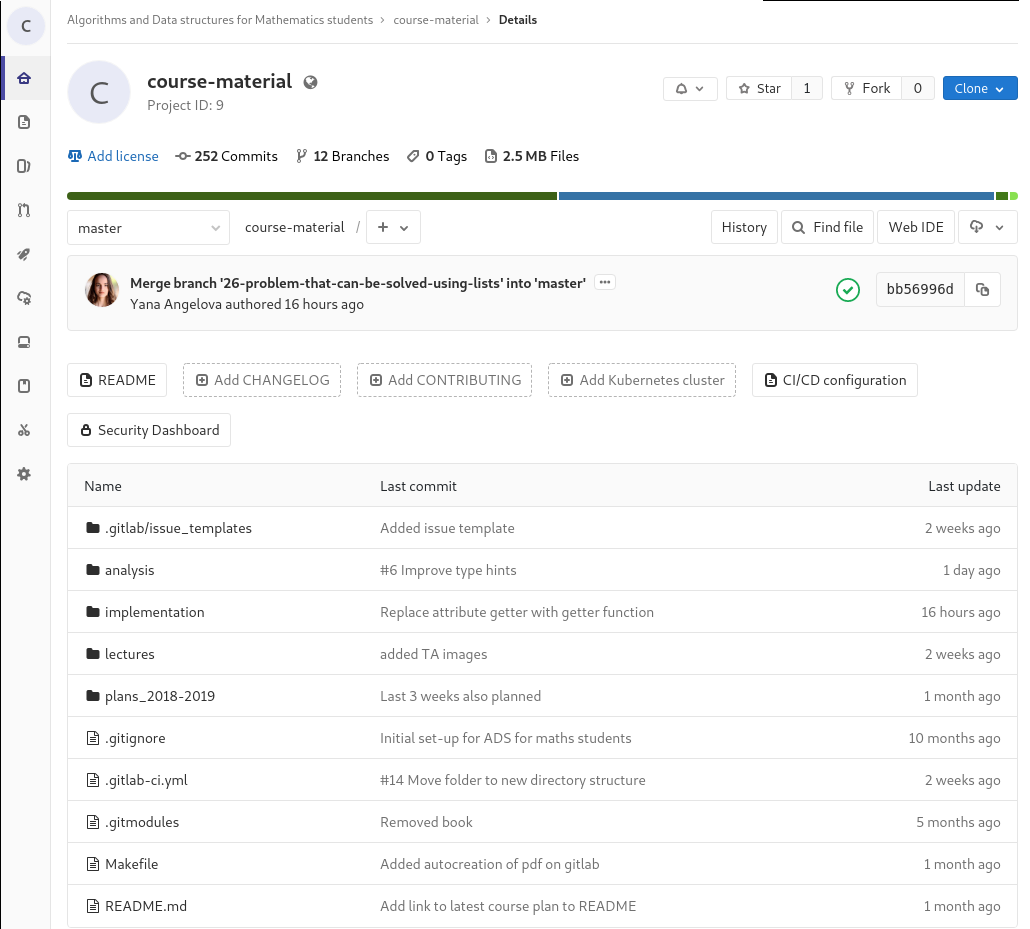
\includegraphics[width=0.8\textwidth]{figures/course-setup.png}\
	\end{center}
\end{frame}

\begin{frame}
	\frametitle{Who?}
	\begin{columns}[t]
		\column{0.505\textwidth}
			\begin{alertblock}{Me}
				\begin{center}
					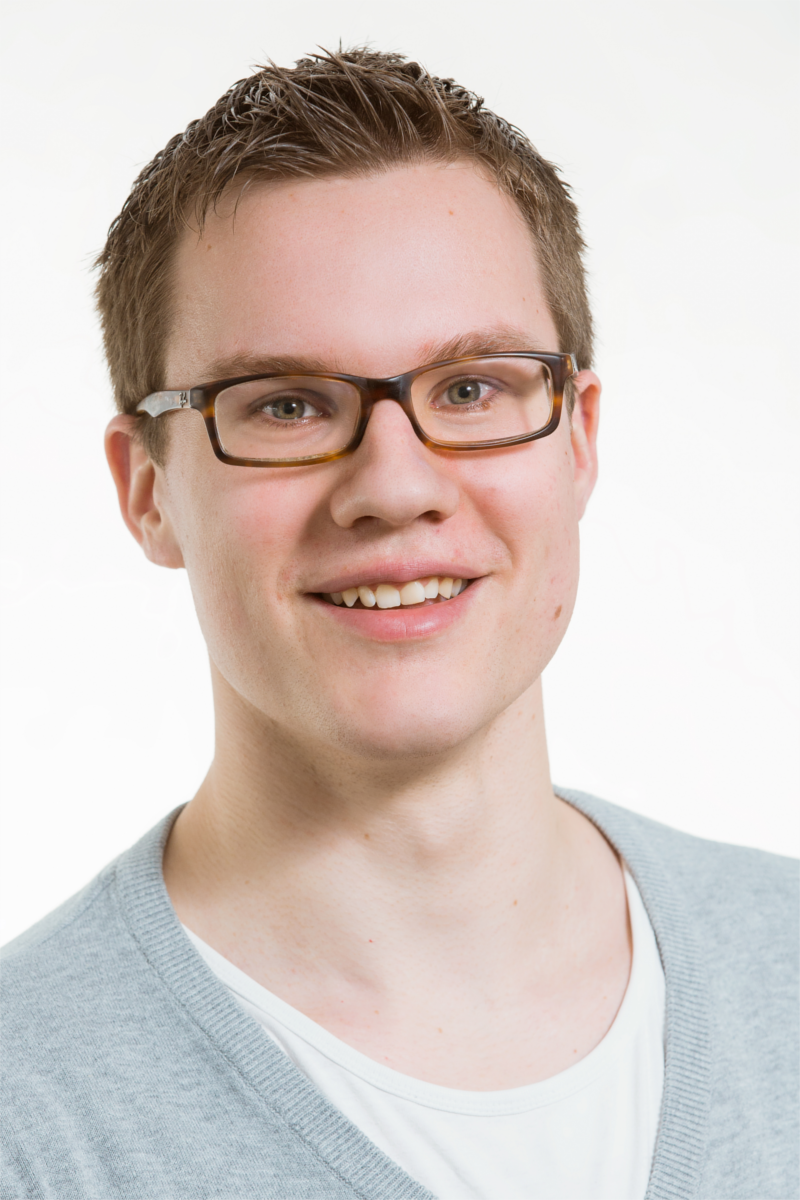
\includegraphics[width=0.4\textwidth]{figures/stefan.png}\\
					Stefan Hugtenburg\\
					Teacher\\
					Computer scientist (not mathematician!)
				\end{center}	
			\end{alertblock}	
		\pause
		\column{0.405\textwidth}
			\begin{exampleblock}{Teaching Assistants}
		\begin{figure}[htpb]
			\begin{subfigure}[]{0.4\textwidth}
			\centering
			
\includegraphics[width=\textwidth]{figures/yoshi.png}\\
			\caption*{Yoshi vd Akker}
			\end{subfigure}
			\hfill
			\begin{subfigure}[]{0.4\textwidth}
			\centering
			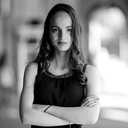
\includegraphics[width=\textwidth]{figures/yana.png}\\
			\caption*{Yana Angelova}
			\end{subfigure}
			\hfill\\
			\begin{subfigure}[]{0.4\textwidth}
			\centering
			
\includegraphics[width=\textwidth]{figures/kevin.png}\\
			\caption*{Kevin Chong}
			\end{subfigure}
			\hfill
			\begin{subfigure}[]{0.4\textwidth}
			\centering
			
\includegraphics[width=\textwidth]{figures/maarten.png}\\
			\caption*{Maarten Sijm}
			\end{subfigure}
			
		\end{figure}
			\end{exampleblock}	
	\end{columns}
\end{frame}

\begin{frame}
	\frametitle{Keep in mind\dots We're computer scientists}
	\framesubtitle{XKCD Purity: \url{https://xkcd.com/435}}
	\begin{center}
		
\includegraphics[width=0.8\textwidth]{figures/purity.png}
	\end{center}
	\pnote{We can do CS stuff, but you are probably better at proofs}
\end{frame}

\begin{frame}
	\frametitle{What and when?}

	Every week (weeks 1-4 and 6-8):
	\pause
	\begin{itemize}
		\item Two lectures of two hours. 
			\begin{itemize}
				\item We treat material both from the book and \textit{not} from the book!
			\pause
				\item\alert<2->{ No need for laptops!}
			\pause
				\item Recorded by collegerama.
				\item Will (likely) only be taught this year.
			\end{itemize}
			\pause
		\item One tutorial of two hours.
			\begin{itemize}
				\item We practice with the material discussed in the lectures.
					\pause
				\item Bring a laptop! First half is programming.
				\item Second half is pen-and-paper.
			\end{itemize}
			\pause
		\item One lab of 4 hours.
			\begin{itemize}
				\item Work on your homework and ask questions to the TAs.
				\item Use the lab to get more feedback on things you are stuck on!
					\pause
				\item We will use \url{https://queue.ewi.tudelft.nl} to handle the questions.
			\end{itemize}
	\end{itemize}
\end{frame}


\begin{frame}
	\frametitle{The book}
	\framesubtitle{Plenty of reading}
	\begin{columns}
		\column{0.455\textwidth}
				\begin{center}
					
\includegraphics[width=0.62\textwidth]{figures/book.jpg}\\
					\hspace*{15pt}\hbox{\scriptsize Photo By:\thinspace{\itshape Stefan Hugtenburg}}\\
					\hspace*{15pt}\hbox{\scriptsize Book cover design by:\thinspace{\itshape Kenji Ngieng}}\\
					\hspace*{15pt}\hbox{\scriptsize Book cover photo by:\thinspace{\itshape Christine Osborne Pictures}}
				\end{center}
		\column{0.555\textwidth}
		\begin{block}{The book}
			Title: Data Structures \& Algorithms in Python.\\
			Authors: 
			\begin{itemize}
				\item M.\ T.\ Goodrich, 
				\item R.\ Tamassia, 
				\item M.\ H.\ Goldwasser
			\end{itemize}
			ISBN: 978-1-118-29027-9
			\end{block}	
			
	\end{columns}
\end{frame}

\begin{frame}
	\frametitle{Weekly assignments}
	\framesubtitle{\url{https://weblab.tudelft.nl}}

	\begin{itemize}
		\item Every week is accompanied by a set of homework assignments.
			\begin{itemize}
				\item Each set should be about 5 to 8 hours of work.
				\item There are strict deadlines (Sunday evening 23:59 at the end of the week).
				\item Assignments are \textit{not} mandatory, but serve as \textit{feedback} assignments.
				\item Experience from the CSE-edition of this course: did not do homework? Fail the course.
			% TODO: [stefan] Check the stats (Fri 04 Jan 2019 05:14:21 PM CET)
			\end{itemize}
		\item Every set consists of implementation assignments (coding!) and analysis assignments (proofs, run time
			analysis, etc).
		\item All assignments are done in WebLab, an online environment that allows you to type python and run tests.
	\end{itemize}
\end{frame}

\begin{frame}
	\frametitle{What is this WebLab?}
	\framesubtitle{\url{https://weblab.tudelft.nl}}

	\begin{itemize}
		\item Let me just show you :)
	\end{itemize}
\end{frame}

\begin{frame}
	\frametitle{Exams (see the studyguide)}
	\framesubtitle{Me asking you questions}

	There are four(!) exams for this course:
	\begin{itemize}
		\item $M_a$ Midterm analysis (week 5), 2 hours: pen-and-paper questions about all the material from week 1 through 4.
		\item $M_i$ Midterm implementation (week 5), 2 hours: computer exam, implementation assignments about all material
			from week 1 through 4.
			\pause
		\item $F_a$ End term analysis (week 9), 2 hours: pen-and-paper questions about all course material.
		\item $F_i$ End term implementation (week 9), 2 hours: computer exam, implementation assignments about all course
			material.
	\end{itemize}
			\pause
	Now take $G = 0.1M_a + 0.1M_i +0.4F_a+0.4F_i$.\\
	Your final grade $F$ is computed as follows:
	\begin{itemize}
		\item If $F_a < 5$: $F= \min(F_a, G)$
		\item If $F_i < 5$: $F= \min(F_i, G)$
		\item Else $F=G$. You pass the course iff $F \geq 5.75$.
	\end{itemize}
	
\end{frame}

\begin{frame}
	\frametitle{Communication}
	\framesubtitle{You asking me questions}

	If you have \textit{content-based} questions, then:
	\begin{itemize}
		\item Come talk to me during lecture breaks or after the lecture/tutorial.
		\item Ask your fellow students!
		\item Post them on the Brightspace forums.
		\item Ask the TAs during the labs.
		\item Content-based questions via e-mail will \textit{not} be answered.
	\end{itemize}

	\hfill\\
	If you have \textit{admin-related} questions, then:
	\begin{itemize}
		\item Ask them during the first 5 minutes of a lecture (which are reserved for those).
		\item E-mail me at \href{mailto:ads-tw-ewi@tudelft.nl}{ads-tw-ewi@tudelft.nl}
		\item E-mails to my personal mailbox will \textit{not} be answered.
	\end{itemize}
\end{frame}

\begin{frame}
	\frametitle{All of the materials}
	\framesubtitle{Help us improve the materials!}

	\begin{itemize}
		\item All materials are publicly available: \url{https://gitlab.ewi.tudelft.nl/ads-maths/course-repository}.
			\pause
		\item This includes:
			\begin{itemize}
				\item These slides \pause (and their TeX sources).
					\pause
				\item All lab assignments \pause (and their solutions).
					\pause
				\item All exams \pause (but only after you have taken them).
					\pause
				\item Course plans and misc. other materials.
			\end{itemize}
			\pause
		\item If you find mistakes in any of the materials, then:
			\begin{itemize}
				\item Point them out to TAs or me. We appreciate it!
					\pause
				\item Create an issue in GitLab. We really like it!  :)
					\pause
				\item Fix them yourself by making a merge request in GitLab. We love it! :D
			\end{itemize}
	\end{itemize}
\end{frame}

\begin{frame}
	\frametitle{Let's get started}
	\framesubtitle{Any questions before we do?}
	\begin{center}
		
\includegraphics[width=0.8\textwidth]{figures/letsgo.jpg}\\
		\hspace*{15pt}\hbox{\scriptsize Image By:\thinspace{\itshape Juhasz Imre}}
		%https://www.pexels.com/photo/123-let-s-go-imaginary-text-704767/
	\end{center}
\end{frame}
